
% !TeX root = ../../main.tex
\subsection{NMAP}
Para a realização de testes de varredura de portas e identificação de serviços, 
foi utilizada a ferramenta Nmap, como mostrado na Figura \ref{fig:nmap1}. Foi utilizado 
o comando \textit{nmap 172.24.30.10}, que realiza uma varredura de portas 
no endereço IP do Host Zabbix. O resultado da varredura indicou 
que as portas 22 (SSH), 80 (HTTP) e 3306 (MySQL) estavam abertas, indicando a presença desses serviços no Host Zabbix.

\begin{figure}[H]
    \centering
    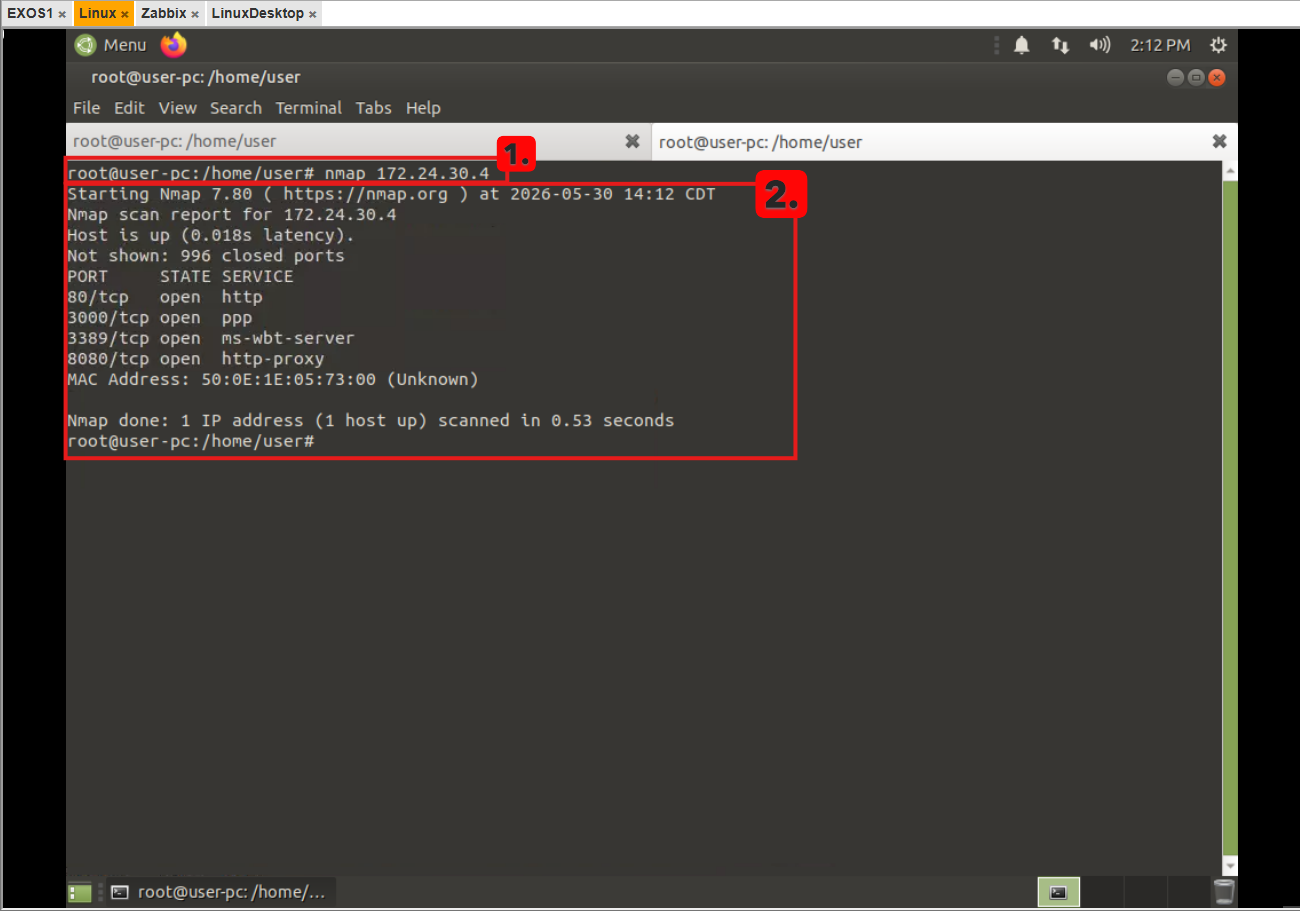
\includegraphics[width=1\linewidth]{fig/nmap/nmap1.png}
    \caption{Varredura de portas utilizando o Nmap; 1. Comando para realizar a varredura de portas no Host Zabbix; 
    2. Resultado da varredura indicando as portas abertas e os serviços correspondentes}
    \label{fig:nmap1}
\end{figure}


Já na Figura \ref{fig:nmap2}, foi utilizado o comando, 
\textit{nmap 172.24.30.4 172.24.30.254}, que realiza uma varredura de portas 
nos endereços IPs 172.24.30.4 e 172.24.30.254, 
o resultado da varredura indicou que as portas
22 (SSH), 80 (HTTP) e 3306 (MySQL) estavam abertas no Host Zabbix, 
enquanto as portas dos outros hosts estavam fechadas, indicando a 
ausência desses serviços nos demais hosts da rede.

\begin{figure}[H]
    \centering
    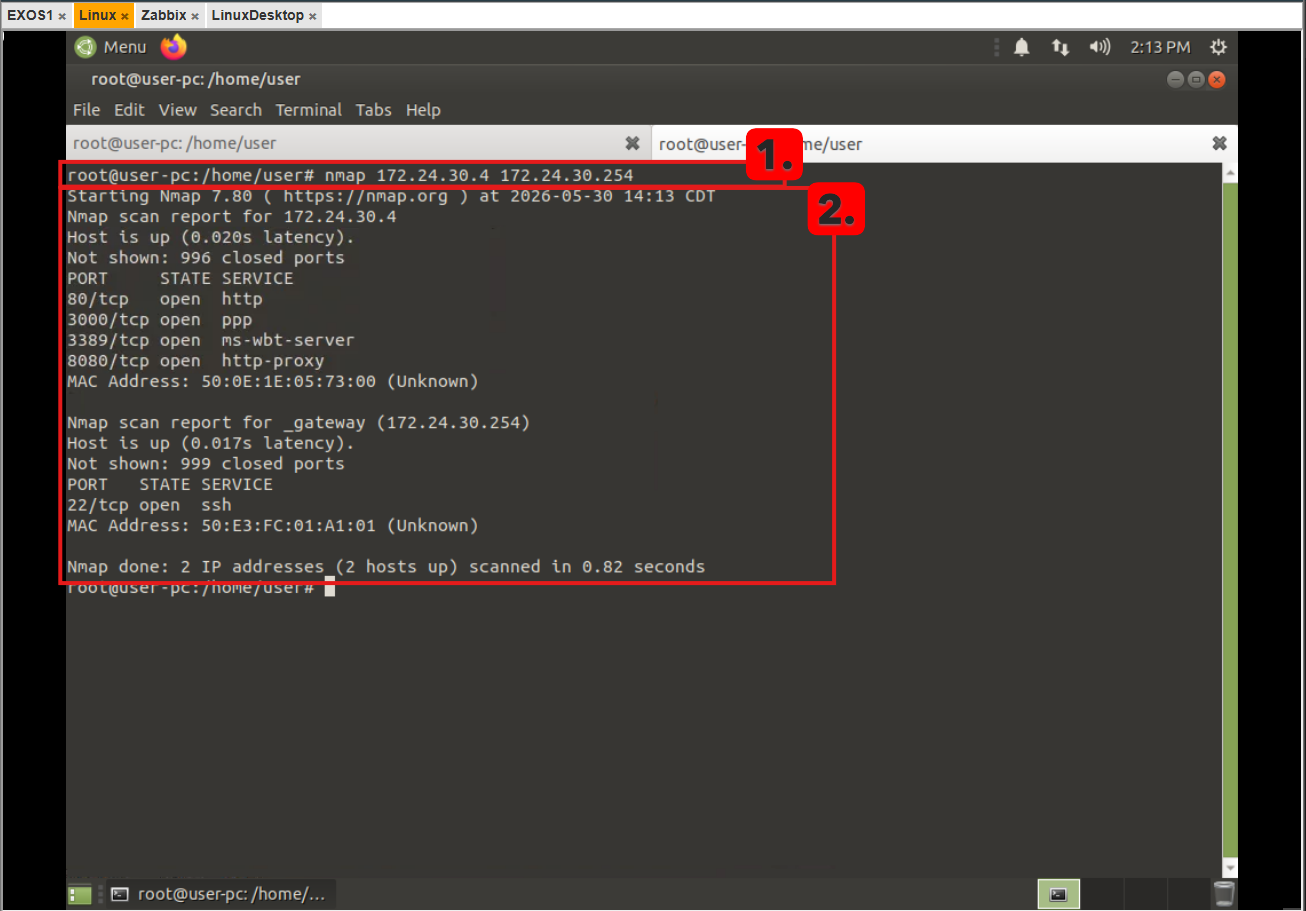
\includegraphics[width=1\linewidth]{fig/nmap/nmap2.png}
    \caption{Varredura de portas utilizando o Nmap; 
    1. Comando para realizar a varredura de portas nos endereços IPs 172.24.30.4 e 172.24.30.254; 
    2. Resultado da varredura indicando as portas abertas e os serviços correspondentes}
    \label{fig:nmap2}
\end{figure}

Em seguida, por meio do comando \textit{nmap 172.24.30.1-254}, 
mostrado na Figura \ref{fig:nmap3}, foi realizada 
uma varredura de portas e identificação de serviços em um intervalo de 
endereços IP, o resultado da varredura indicou três endereços IP disponíveis na rede, 
sendo eles 172.24.30.14, 172.24.30.254 e 172.24.30.10. Além disso, a varredura indicou
 quais portas estavam abertas em cada um dos hosts, 
 bem como os serviços correspondentes a essas portas.

\begin{figure}[H]
    \centering
    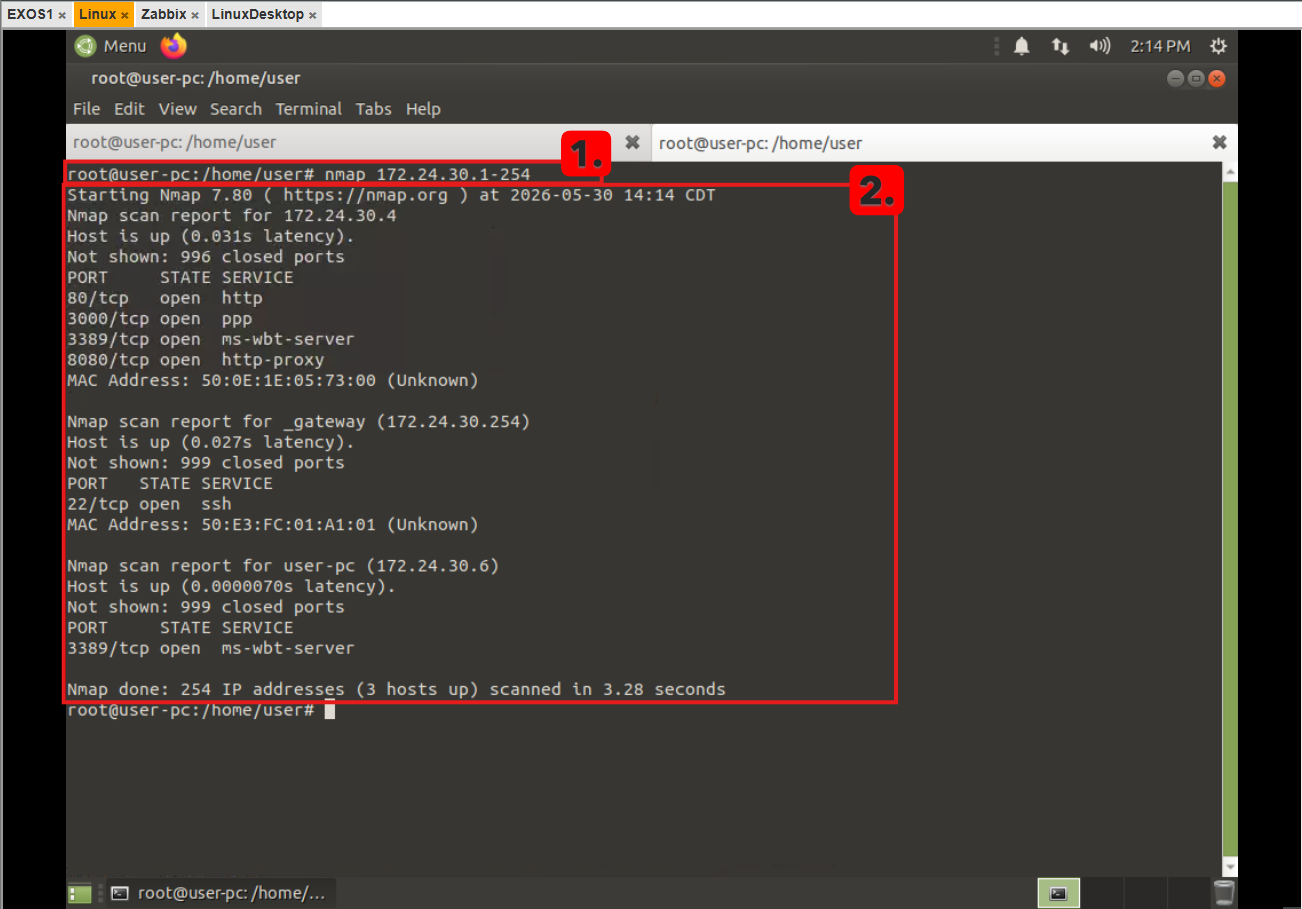
\includegraphics[width=1\linewidth]{fig/nmap/nmap3.png}
    \caption{Varredura de portas utilizando o Nmap; 1. Comando para realizar a varredura de portas em um intervalo de endereços IP; 
    2. Resultado da varredura indicando os endereços IP disponíveis na rede, as portas abertas e os serviços correspondentes}
    \label{fig:nmap3}
\end{figure}


Já na Figura \ref{fig:nmap4}, foi utilizado o comando \textit{nmap 172.24.30.254 -sS}, 
que realiza uma varredura de portas utilizando o método de varredura TCP SYN,
 o resultado da varredura indicou que a porta 22 (SSH) estava aberta no gateway e mostrou o MAC Address.

\begin{figure}[H]
    \centering
    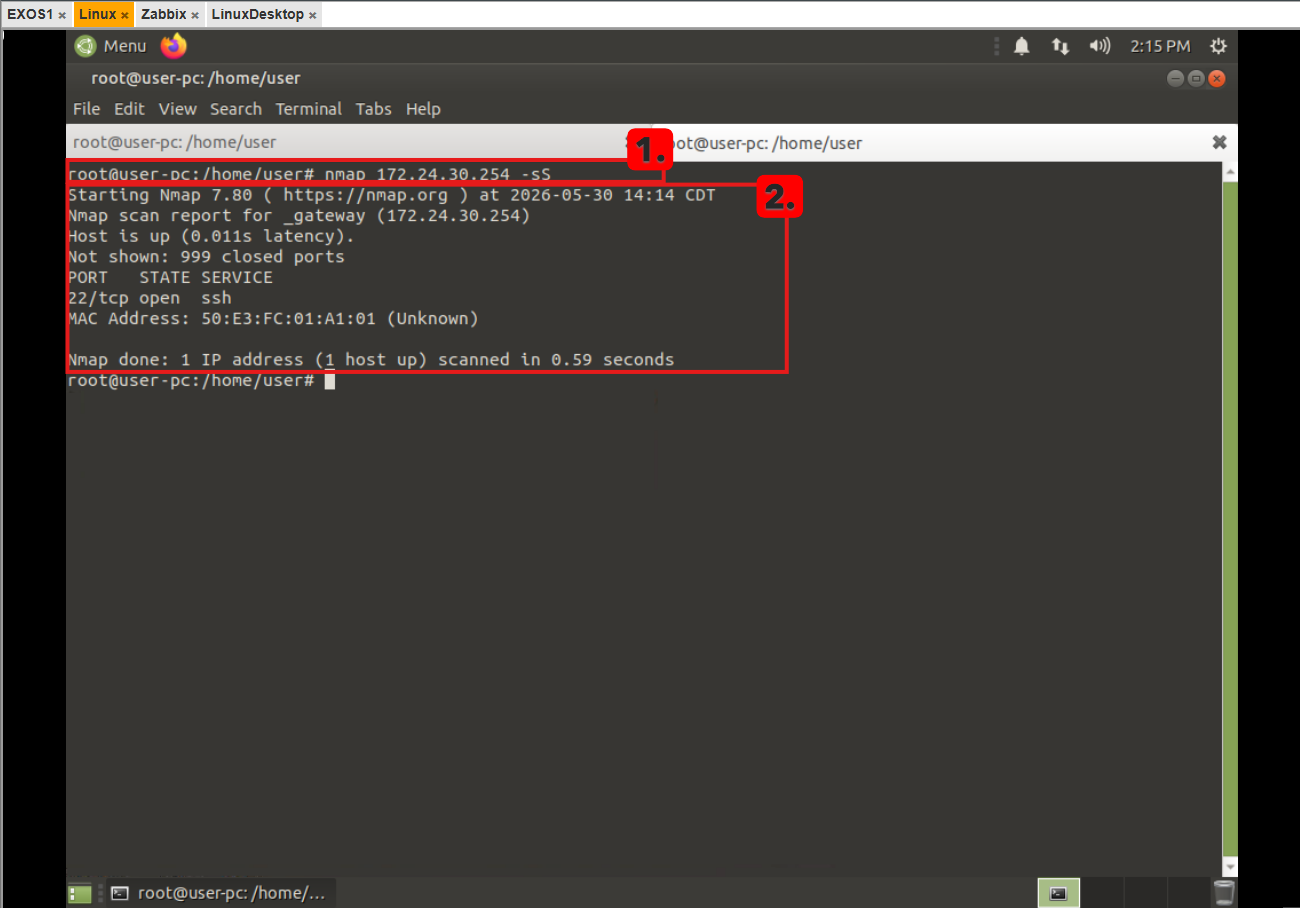
\includegraphics[width=1\linewidth]{fig/nmap/nmap4.png}
    \caption{Varredura de portas utilizando o Nmap; 
    1. Comando para realizar a varredura de portas utilizando o método de varredura TCP SYN; 
    2. Resultado da varredura indicando as portas abertas e os serviços correspondentes}
    \label{fig:nmap4}
\end{figure}

Em seguida, por meio do comando \textit{nmap 172.24.30.1-254 -sV}, mostrado na Figura \ref{fig:nmap5},\ref{fig:nmap6} e \ref{fig:nmap7}, 
foi realizada uma varredura de portas e identificação do tipo de serviços utilizando o método de varredura 
TCP SYN em um intervalo de endereços IP, o resultado da varredura indicou quais IPs estavam disponíveis 
na rede, quais portas estavam abertas em cada um dos hosts, 
bem como os serviços e a versão dos serviços correspondentes a essas portas.


\begin{figure}[H]
    \centering
    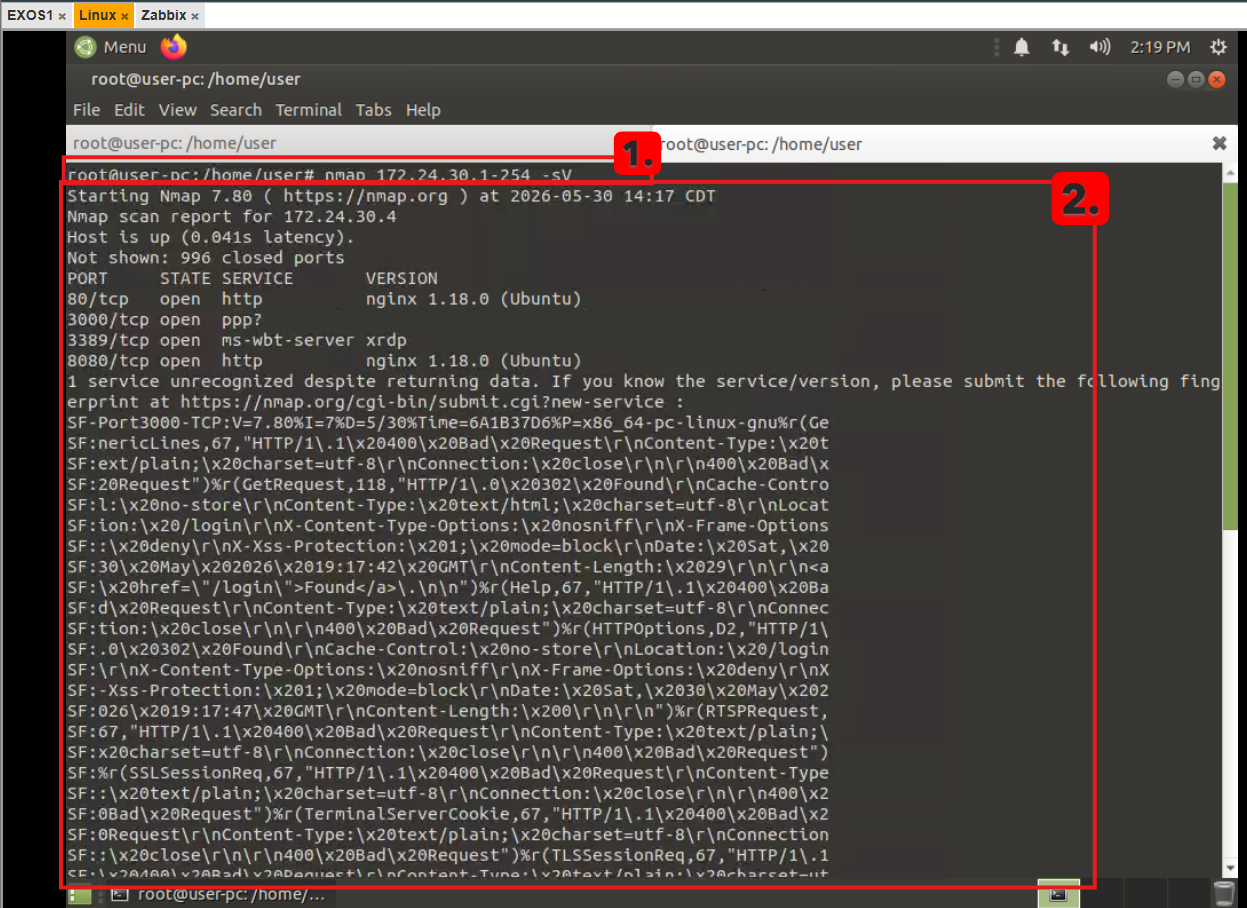
\includegraphics[width=1\linewidth]{fig/nmap/nmap5.png}
    \caption{Varredura de portas utilizando o Nmap 1; 
     1. Comando para realizar a varredura de portas e identificação do tipo de serviços;
     2. Resultado da varredura indicando os endereços IP disponíveis na rede }
    \label{fig:nmap5}
\end{figure}


\begin{figure}[H]
    \centering
    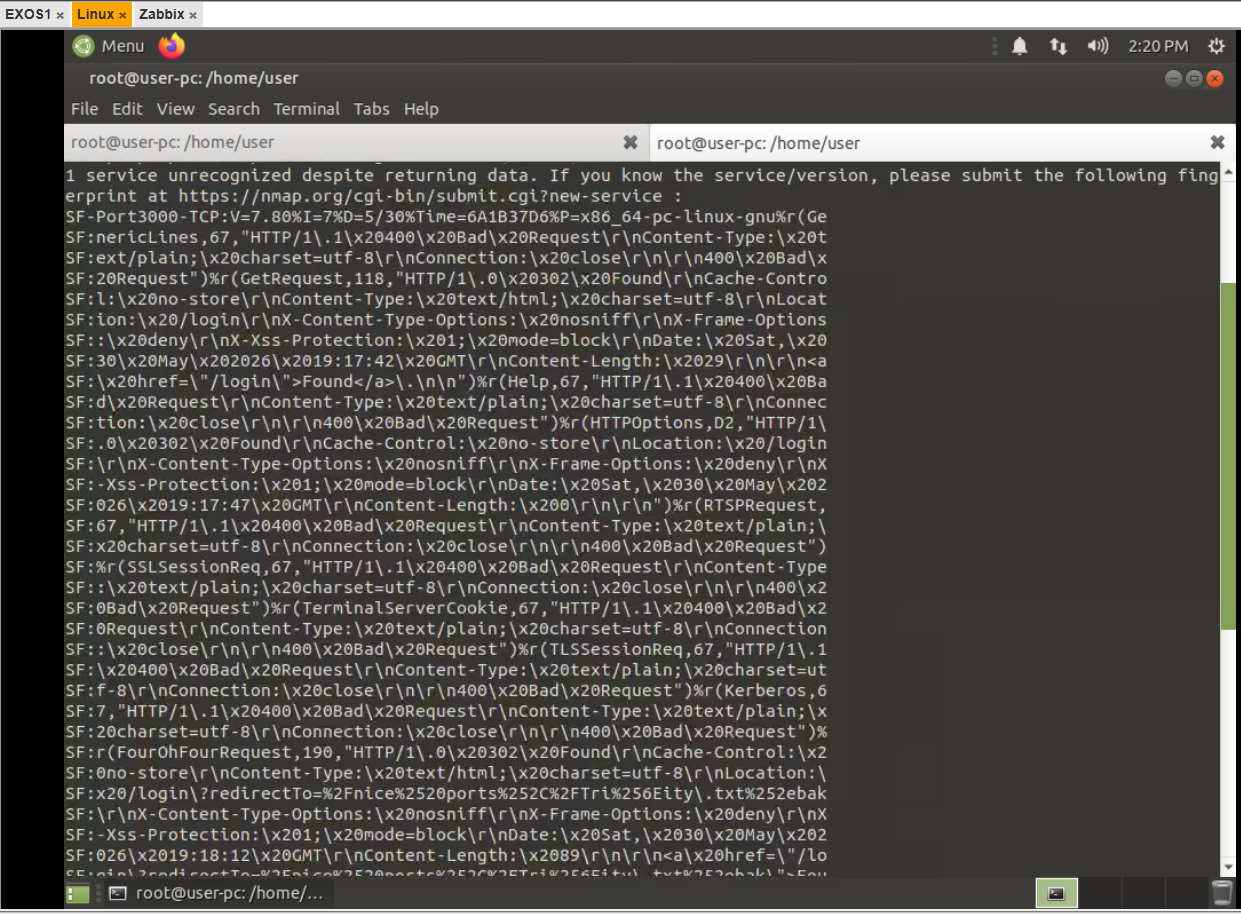
\includegraphics[width=1\linewidth]{fig/nmap/nmap6.png}
    \caption{Resultado da varredura utilizando o Nmap 2}
    \label{fig:nmap6}
\end{figure}

\begin{figure}[H]
    \centering
    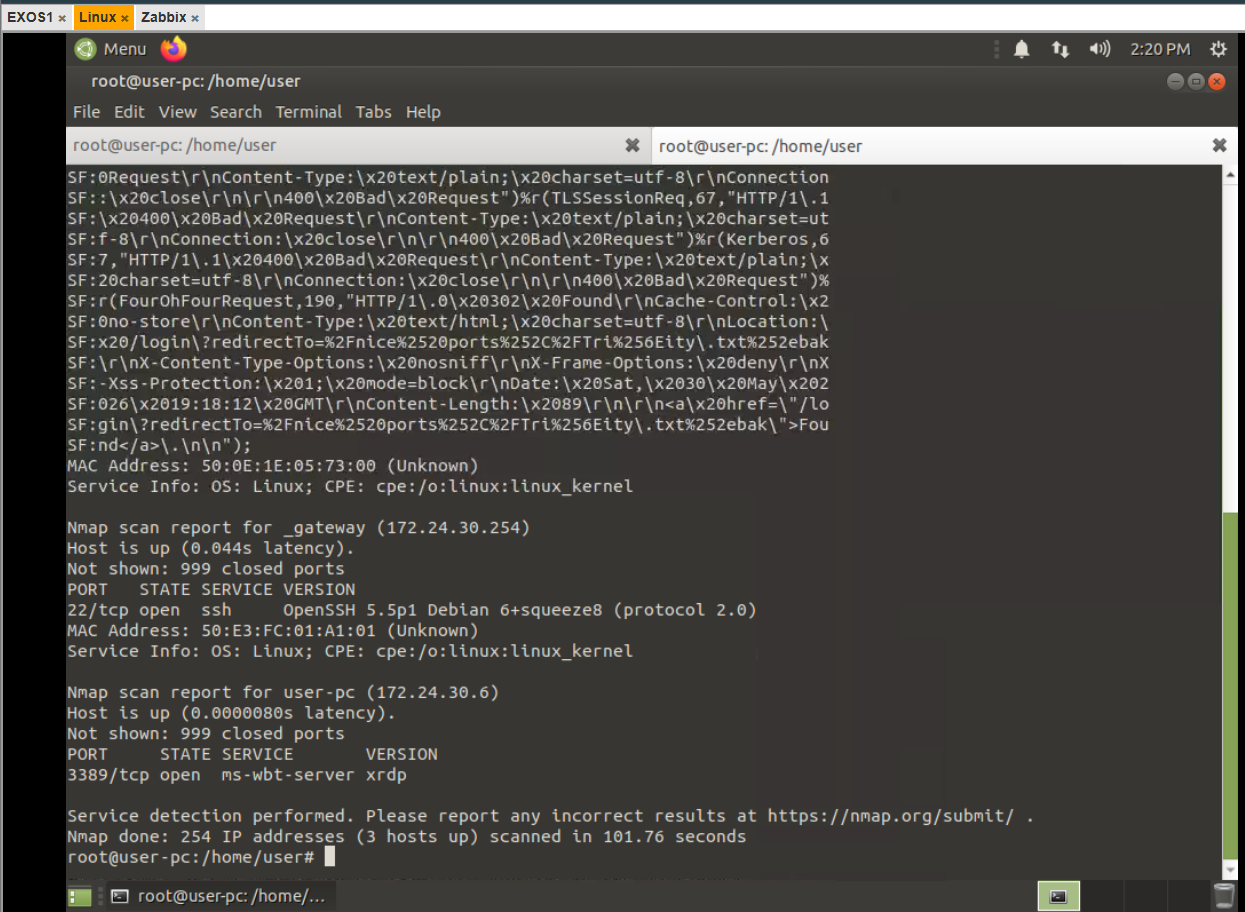
\includegraphics[width=1\linewidth]{fig/nmap/nmap7.png}
    \caption{Resultado da varredura utilizando o Nmap 3}
    \label{fig:nmap7}
\end{figure}

Como última simulação, foi utilizado o comando \textit{nmap 172.24.30.254 -A}. Por meio desse comando, é possível 
detectar o SO, a versão, verificar scripts e traceroute. Como resultado da varredura, 
foi possível identificar o sistema operacional do gateway, a versão do serviço SSH,
 bem como a presença de scripts de segurança e o caminho de rede para o host alvo.

\begin{figure}[H]
    \centering
    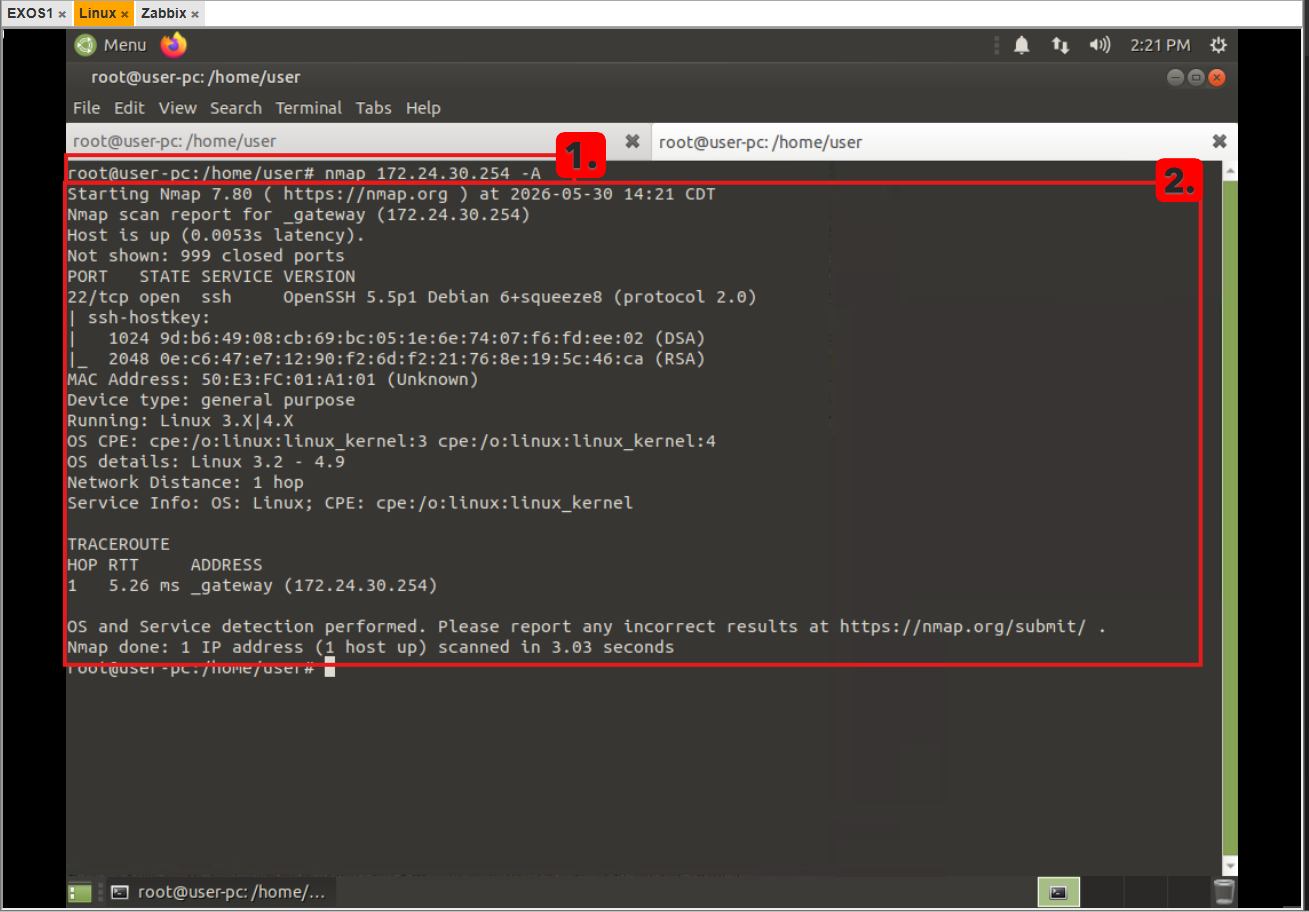
\includegraphics[width=1\linewidth]{fig/nmap/nmap8.png}
    \caption{Resultado da varredura utilizando o Nmap com a opção -A; 
    1. Comando para realizar a varredura de portas e identificação do tipo de serviços utilizando a opção -A; 
    2. Resultado da varredura indicando o sistema operacional, a versão do serviço SSH}
    \label{fig:nmap8}
\end{figure}